\documentclass[10pt]{article}
\usepackage[T1]{fontenc}
\usepackage{lmodern,amsmath,amssymb,graphicx,hyperref}
\usepackage[margin=.75in]{geometry}
\setlength{\parindent}{0pt}\setlength{\parskip}{6pt}
\begin{document}
\begin{center}{\Large Degree-limited actual whole-chart factors}\\[4pt]
14 November 2026; local29 statements; data PCC-20261114-36a2d2
\end{center}
\textbf{Local construction.} Accepted draft004/build004 elaborates29
statements,exit0/no warnings. This separate draft is OUTSIDE Compact39's
shared audit and fresh replay. Five central printed dependencies contain
only standard foundations. All observations are unsigned [pcc:unverified].

\textbf{Actual scope.} Use the same completed auxiliary $W$, actual bounded
ports $x,y<2^a$, natural multiplicities, and nonzero signed-grid source node
$t$ with $v_2(t)=i<u\le a$. Matrices explicitly mask noncrossing entries to
zero. The actual fixed negative-pole diagonal is $c$, with $w=v_2(c)$.
No positive multiplicity or nonzero local-first-jet premise is added.

\textbf{Combined grading.} Coefficient $H^b$ of the actual bivariate
geometric approximation has $Z$-grade $b-1$. Dividing by $2^b$ gives
grade $-1$ of the actual constructed right factor $V_{(r,b),y}(Z)$:
\[
 v_2([Z^n]V_{(r,b),y})\ge n-1,
\]
with zero coefficients admitted at every weight. The grade is derived from
actual denominator slopes and the existing actual normalized chart, rather
than supplied as a good-factor hypothesis [pcc:unverified].

Define $V^{\le k}$ by truncating each actual right polynomial below degree
$k+1$. The coefficient bound gives content-$k$ error. The finite matrix
product error is proved using actual left integrality and sums, then scaled
by $c$. The resulting profile is
\[
 \begin{gathered}
 \operatorname{natdeg}V^{\le k}_{(r,b),y}\le k,\qquad
 \operatorname{Content}_0(V^{\le k}_{(r,b),y}),\\
 \operatorname{Content}_{w+b}(\widehat U_{x,(r,b)}),\qquad
 \operatorname{Content}_{w+k}
   (W^{\rm cross}_{xy}-(\widehat U V^{\le k})_{xy}),\\
 \#\{(r,b)\}=2^u k.
 \end{gathered}
\]
Every label remains charged; $k=0$ is included. Scaled-left integrality
retains $w\ge0$. No full-matrix or origin rank claim [pcc:unverified].

\begin{center}
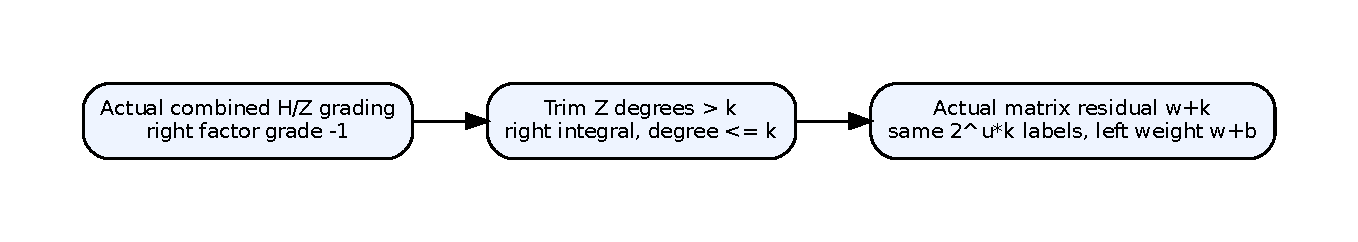
\includegraphics[width=\linewidth,height=1.15in,keepaspectratio]{dependencies.pdf}
\end{center}
\textbf{Evidence and failures.} Exact accepted source/log/exit are pinned in
local-validation-002.json; prior21 data is PCC-20261114-20c45d. All four
drafts/raw builds are retained. Failures include a reserved-lambda variable,
an omitted unfolding and ambiguous weightedLeft. Accepted004 has no
\texttt{sorryAx}; no linter or acceptance condition was disabled
[pcc:unverified].

\textbf{Next discrimination.} Independent promotion/audit/replay remains
pending. Degree and labels do not price coefficient construction, bit sizes,
entry or creation precision, original mode density, recovery, recursion,
actual elliptic relation/public finder/extraction/retry/expected bit cost.
Read exact Mixed/Graded, actual Compact and pinned PowerSeries truncation
APIs before this derivation; KB unavailable as journaled. Standard algebra
is reused without a novelty or speed claim. No native crypto, solver,
timing, paid or cloud experiment; all parent pins remain exact.
\end{document}
